% Manuscript derived from the IEEEtran bare conference template.
% The unmodified upstream template is preserved under ieee-template/vendor/.
\documentclass[conference]{ieee-template/vendor/IEEEtran/IEEEtran}

\usepackage{cite}
\usepackage{amsmath,amssymb}
\usepackage{graphicx}
\usepackage{booktabs}
\usepackage{flafter}
\usepackage{url}
\usepackage[hidelinks]{hyperref}

\graphicspath{{figures/}}

\title{Compute-Constrained Road Damage Detection across Geographic and Sensor Domains}

% An anonymized version can be generated later if required by the target venue.
\author{\IEEEauthorblockN{Mateus Gomes de Ara\'{u}jo}
\IEEEauthorblockA{Computer Engineering\\
University of Bras\'{i}lia (UnB)\\
Bras\'{i}lia, Brazil\\
mathweuzz@gmail.com}}

\begin{document}

\maketitle

\begin{abstract}
Road damage detection systems are commonly evaluated using pooled benchmarks,
although deployment conditions vary across countries, sensors, resolutions,
and road environments. This paper studies multidomain road damage detection on
RDD2022 under a reproducible CPU-only budget. A leakage-aware protocol groups
nearby frames, preserves negative images, and yields 38,385 labeled images with
55,006 valid instances. A 2.59-million-parameter YOLO11n detector is fine-tuned
for 10 epochs on an equal-domain subset of 2,800 images in 28.5 minutes. On the
held-out 3,703-image test split, it obtains 3.26\% COCO mAP and 8.51\% AP50 at
43.4 images/s. Domain mAP ranges from 0.42\% for Norway to 6.11\% for the United
States, while small-object AP is only 0.26\%. At a 0.25 score threshold, 0.92\%
of negative images produce a false detection. These results quantify the sharp
accuracy cost of an extreme CPU and data budget and show why pooled accuracy
alone is insufficient for assessing deployment reliability.
\end{abstract}

\begin{IEEEkeywords}
road damage detection, object detection, compute-constrained learning,
multi-domain evaluation, computer vision, RDD2022
\end{IEEEkeywords}

\section{Introduction}
Timely road-condition assessment is necessary for maintenance prioritization,
yet manual surveys are costly to repeat at network scale. Images collected with
smartphones and other widely available cameras provide a lower-cost sensing
alternative, and modern object detectors can localize multiple damage types in
a single pass \cite{maeda2018road}. Deployment reliability, however, depends on
more than aggregate benchmark accuracy. Geographic appearance, pavement and
marking standards, weather, acquisition platform, viewpoint, and image
resolution may change simultaneously between training and operation.

RDD2022 provides a useful setting for studying this problem because it combines
road imagery from seven acquisition domains spanning six countries
\cite{arya2022rdd2022,arya2024rdd2022}. However, an aggregate score can conceal
failure on a particular geography or sensor. Furthermore, a random image-level
partition may place nearby frames from the same acquisition sequence in both
training and evaluation sets, producing an optimistic estimate of deployment
performance. Domain-dependent differences in class frequency, damage scale,
and negative-image prevalence further complicate the comparison.

We address three research questions: \emph{RQ1}, what detection quality is
attainable with a compact model under a fully specified CPU-only budget;
\emph{RQ2}, how strongly does performance vary across the seven geographic and
acquisition domains after equal-domain training; and \emph{RQ3}, which classes,
object scales, and negative-image conditions dominate the remaining errors?

This work therefore focuses on transparent compute constraints and domain-aware
evaluation rather than only aggregate detection accuracy. Its contributions are:
\begin{itemize}
    \item an audited cleaning pipeline and a deterministic, sequence-blocked
    partition of RDD2022 in COCO and YOLO formats;
    \item a deterministic CPU-budgeted baseline trained on an equal-domain
    subset with domain-specific negative prevalence preserved;
    \item domain-, class-, scale-, and negative-image-aware analysis rather
    than reliance on a single pooled score;
    \item a reproducible account of detection accuracy, latency, memory, and
    the accuracy cost imposed by compact CPU-only training.
\end{itemize}

\section{Related Work}
\label{sec:related-work}

\subsection{Road Damage Detection Benchmarks}
Maeda et al. established an early large-scale benchmark for smartphone-based
road inspection, releasing 9,053 images with 15,435 annotated damage instances
and comparing convolutional object detectors for both server and mobile
execution \cite{maeda2018road}. RDD2020 subsequently expanded the task from
Japan to India and the Czech Republic, standardized four damage categories,
and provided 26,336 images for multinational evaluation
\cite{arya2021rdd2020}. A companion study evaluated multiple combinations of
country-specific training and test data and reported substantial degradation
when models trained on Japanese roads were transferred to other countries
\cite{arya2021multiple}.

RDD2022 extends this lineage to 47,420 images from six countries and introduces
additional acquisition shifts, including motorbike, drone, high-resolution
camera, and street-view imagery \cite{arya2024rdd2022}. The associated
CRDDC'2022 attracted solutions dominated by YOLO, Faster R-CNN, and detector
ensembles; the best combined submission achieved an F1 score of approximately
76\% \cite{arya2022crddc}. These results demonstrate the value of model and
data diversity, but leaderboard performance on the provided test sets does not
by itself quantify domain-specific reliability under a fixed low-compute
training procedure.

\subsection{Detection Architectures}
Dense one-stage detectors offer a practical accuracy--cost trade-off for road
inspection. RetinaNet introduced focal loss to reduce the influence of easy
background examples under extreme foreground--background imbalance
\cite{lin2017focal}. Two-stage Faster R-CNN variants instead separate region
proposal from region classification and retain an explicit objectness loss.
The YOLO family emphasizes single-pass prediction and compact deployment. We
use YOLO11n through the versioned Ultralytics implementation
\cite{jocher2025ultralytics}; its 2.6 million parameters make repeated CPU
optimization practical, while the low-resolution Faster R-CNN MobileNetV3
variant serves as an engineering qualification control. This choice targets a
reproducible resource regime, not a state-of-the-art leaderboard claim.

\subsection{Cross-Domain Robustness}
Cross-country road damage detection has been studied through both pooled
multinational training and domain adaptation. DA-RDD, for example, aligns
image- and instance-level features between a labeled source and an unlabeled
target domain \cite{lin2023darDD}. This setting differs from domain
generalization: adaptation uses target-domain samples during training, whereas
generalization requires deployment to a domain that was unavailable during
model fitting and selection. More broadly, Domain Generalised Faster R-CNN
regularizes both classification and localization under domain shift
\cite{seemakurthy2023dgfrcnn}. DomainBed further shows that fair conclusions
depend on consistent architectures, tuning budgets, and model-selection rules,
and that a carefully implemented empirical-risk-minimization baseline can be
difficult to outperform \cite{gulrajani2021domainbed}.

Following these lessons, our study establishes a controlled empirical-risk
minimization baseline under a fixed CPU budget. Its distinguishing focus is not
a new adaptation loss, but a sequence-aware, equal-domain assessment that
preserves negative images and reports domain-level rather than only pooled
performance. We deliberately avoid interpreting domain slices as unseen-domain
generalization.

\section{Problem Formulation}
\label{sec:formulation}

\subsection{Multi-Domain Object Detection}
Let $\mathcal{D}=\{1,\ldots,D\}$ denote the acquisition domains, with $D=7$,
and let
\begin{equation}
 \mathcal{Z}_d=\{(x_{di},Y_{di})\}_{i=1}^{n_d},\quad
 Y_{di}=\{(b_{dij},c_{dij})\}_{j=1}^{m_{di}},
 \label{eq:domain-data}
\end{equation}
where $x_{di}\in\mathbb{R}^{H_i\times W_i\times3}$, normalized box
$b_{dij}\in[0,1]^4$, and $c_{dij}\in\mathcal{C}=\{\mathrm{D00},
\mathrm{D10},\mathrm{D20},\mathrm{D40}\}$. A negative image is represented
without a synthetic background box, i.e., $Y_{di}=\varnothing$ and $m_{di}=0$.
A detector maps an image to $K$ scored hypotheses,
\begin{equation}
 f_\theta(x)=\{(\hat b_k,\hat{\boldsymbol p}_k)\}_{k=1}^{K},
 \qquad \hat{\boldsymbol p}_k\in[0,1]^{|\mathcal C|}.
 \label{eq:detector}
\end{equation}

Let $\mathcal A_i$ be the multiscale candidate locations for image $i$. For
candidate $a$ and target $j$, the task-alignment score is
\begin{equation}
 t_{iaj}=p_{ia,c_j}^{\alpha}
 \operatorname{IoU}(\hat b_{ia},b_{ij})^{\beta},
 \label{eq:task-alignment}
\end{equation}
and $\mathcal P_i$ contains the top-$k$ candidates for each target whose centers
fall inside that target. The selected alignment values are normalized into soft
class targets $s_{iac}\in[0,1]$. For Bernoulli cross-entropy
$\operatorname{BCE}(p,s)=-s\log p-(1-s)\log(1-p)$, classification is
\begin{equation}
 L_{\mathrm{cls}}=\sum_i\sum_{a\in\mathcal A_i}
 \sum_{c\in\mathcal C}\operatorname{BCE}(p_{iac},s_{iac}).
 \label{eq:yolo-cls}
\end{equation}
Thus, when $Y_i=\varnothing$, every $s_{iac}=0$: localization vanishes but
background classification remains active.

For a continuous target distance $y\in[0,R-1)$ and categorical distribution
$q\in\Delta^{R-1}$, let $l=\lfloor y\rfloor$ and
$u=\min(l+1,R-1)$. The
distribution focal loss is
\begin{equation}
 \operatorname{DFL}(q,y)=-(u-y)\log q_l-(y-l)\log q_u.
 \label{eq:dfl}
\end{equation}
With $Z=\max(\sum_{i,a,c}s_{iac},1)$ and matched target $\mu(i,a)$, the frozen
YOLO objective is represented by
\begin{multline}
 \mathcal L(\theta)=\frac{\lambda_{\mathrm{cls}}}{B}L_{\mathrm{cls}}\\
 +\frac{1}{Z}\sum_i\sum_{a\in\mathcal P_i}
 s_{ia,c_{\mu(i,a)}}\Bigg[\lambda_{\mathrm{box}}\\
 \cdot\bigl(1-\operatorname{CIoU}(
 \hat b_{ia},b_{i\mu(i,a)})\bigr)
 +\lambda_{\mathrm{dfl}}\sum_{r\in\{l,t,r,b\}}
 \operatorname{DFL}(q_{iar},y_{iar})\Bigg],
 \label{eq:yolo-loss}
\end{multline}
where $(\lambda_{\mathrm{box}},\lambda_{\mathrm{cls}},
\lambda_{\mathrm{dfl}})=(7.5,0.5,1.5)$ and $B$ is batch size. This exposes how
classification, geometry, and discretized boundary regression compete under a
fixed optimization budget.

\subsection{Domain Risk and Negative Prevalence}
For loss $\ell$, the empirical domain risk and a weighted source risk are
\begin{equation}
 \widehat R_d(\theta)=\frac{1}{n_d}\sum_{i=1}^{n_d}
 \ell(f_\theta(x_{di}),Y_{di}),\qquad
 \widehat R_{\mathcal S}^{\boldsymbol\alpha}(\theta)=
 \sum_{d\in\mathcal S}\alpha_d\widehat R_d(\theta),
 \label{eq:domain-risk}
\end{equation}
where $\alpha_d=n_d/\sum_{s\in\mathcal S}n_s$ recovers natural pooled sampling
and $\alpha_d=1/|\mathcal S|$ gives equal domain weight. If
$q_d=n_d^{-1}\sum_i\mathbf 1[m_{di}=0]$, then
\begin{equation}
 \widehat R_d=(1-q_d)\widehat R_d^+ +q_d\widehat R_d^-,
 \label{eq:negative-risk}
\end{equation}
making domain-dependent negative prevalence an explicit change in the risk
mixture rather than a secondary dataset statistic.

Let the CPU training budget be $B_{\mathrm{tr}}=2800$ images and define domain
quotas $B_d\in\{\lfloor B_{\mathrm{tr}}/D\rfloor,
\lceil B_{\mathrm{tr}}/D\rceil\}$ such that $\sum_dB_d=B_{\mathrm{tr}}$.
For binary selection $z_{di}$ and negative prevalence $q_d$, the sampler obeys
\begin{equation}
\begin{aligned}
 &\sum_i z_{di}=B_d,\qquad
 \sum_i z_{di}\mathbf 1[m_{di}=0]=\operatorname{round}(q_dB_d),\\
 &\widehat R_{\mathrm{bal}}(\theta)=\frac1D\sum_{d=1}^D
 \frac1{B_d}\sum_i z_{di}\ell(f_\theta(x_{di}),Y_{di}).
\end{aligned}
 \label{eq:balanced-budget}
\end{equation}
The frozen run uses $B_d=400$ for every domain and $E=10$ epochs, hence
$EB_{\mathrm{tr}}=28{,}000$ image presentations. Besides pooled AP, we report
\begin{equation}
 AP_{\mathrm{macro}}=D^{-1}\sum_{d=1}^D AP_d(\theta),\qquad
 AP_{\mathrm{worst}}=\min_d AP_d(\theta),
 \label{eq:macro-worst}
\end{equation}
so a large domain cannot conceal failure on a smaller one. These are
domain-sliced in-distribution results; they are not estimates of adaptation or
unseen-domain generalization.

\subsection{Constrained Sequence-Block Partition}
Within each domain, let $\mathcal G$ be the sequence blocks and define the
feature vector
\begin{equation}
 v_g=(N_g,N_g^-,N_g^{\mathrm{D00}},N_g^{\mathrm{D10}},
 N_g^{\mathrm{D20}},N_g^{\mathrm{D40}})^\top\in\mathbb N^6.
\end{equation}
For split $r\in\{\mathrm{tr},\mathrm{va},\mathrm{te}\}$, binary assignment
$a_{gr}$, target ratio $\rho=(0.8,0.1,0.1)$, total $V=\sum_gv_g$, and
$w=(10,2,3,3,3,3)$, set
\begin{align}
 A_{rk}&=\sum_{g\in\mathcal G}a_{gr}v_{gk}, & T_{rk}&=\rho_rV_k,\\
 \delta_{rk}&=\frac{A_{rk}-T_{rk}}{\max(T_{rk},1)}, &
 o_{rk}&=\frac{[A_{rk}-1.08T_{rk}]_+}{\max(T_{rk},1)}.
\end{align}
The implemented assignment approximately solves
\begin{equation}
\begin{aligned}
 \min_a\quad &J(a)=\sum_{r,k}w_k(\delta_{rk}^2+3o_{rk}^2),\\
 \mathrm{s.t.}\quad &a_{gr}\in\{0,1\},\qquad
 \sum_ra_{gr}=1.
\end{aligned}
 \label{eq:split-objective}
\end{equation}
Rare blocks are greedily placed first using a seed-stable order, after which
30,000 seeded pairwise-swap proposals are accepted only when they decrease
$J$. The constraint in \eqref{eq:split-objective} makes sequence leakage
impossible by construction, while the asymmetric $o_{rk}$ term discourages
overshooting any target feature by more than 8\%.

\section{Dataset and Exploratory Analysis}
\label{sec:dataset}

\subsection{RDD2022}
RDD2022 contains 47,420 road images collected in China, the Czech Republic,
India, Japan, Norway, and the United States \cite{arya2022rdd2022}. China is
represented by two acquisition domains, drone and motorbike, resulting in seven
domains overall. The official task uses four damage categories: longitudinal
cracks (D00), transverse cracks (D10), alligator cracks (D20), and potholes
(D40).

The released data contain 38,385 labeled training images and 9,035 unlabeled
challenge-test images. We found 65,712 annotated objects before cleaning. Of
these, 55,007 belong to the four official classes and 10,705 use additional
labels. One official bounding box has zero width and is removed, leaving 55,006
valid target instances.

\begin{figure*}[t]
    \centering
    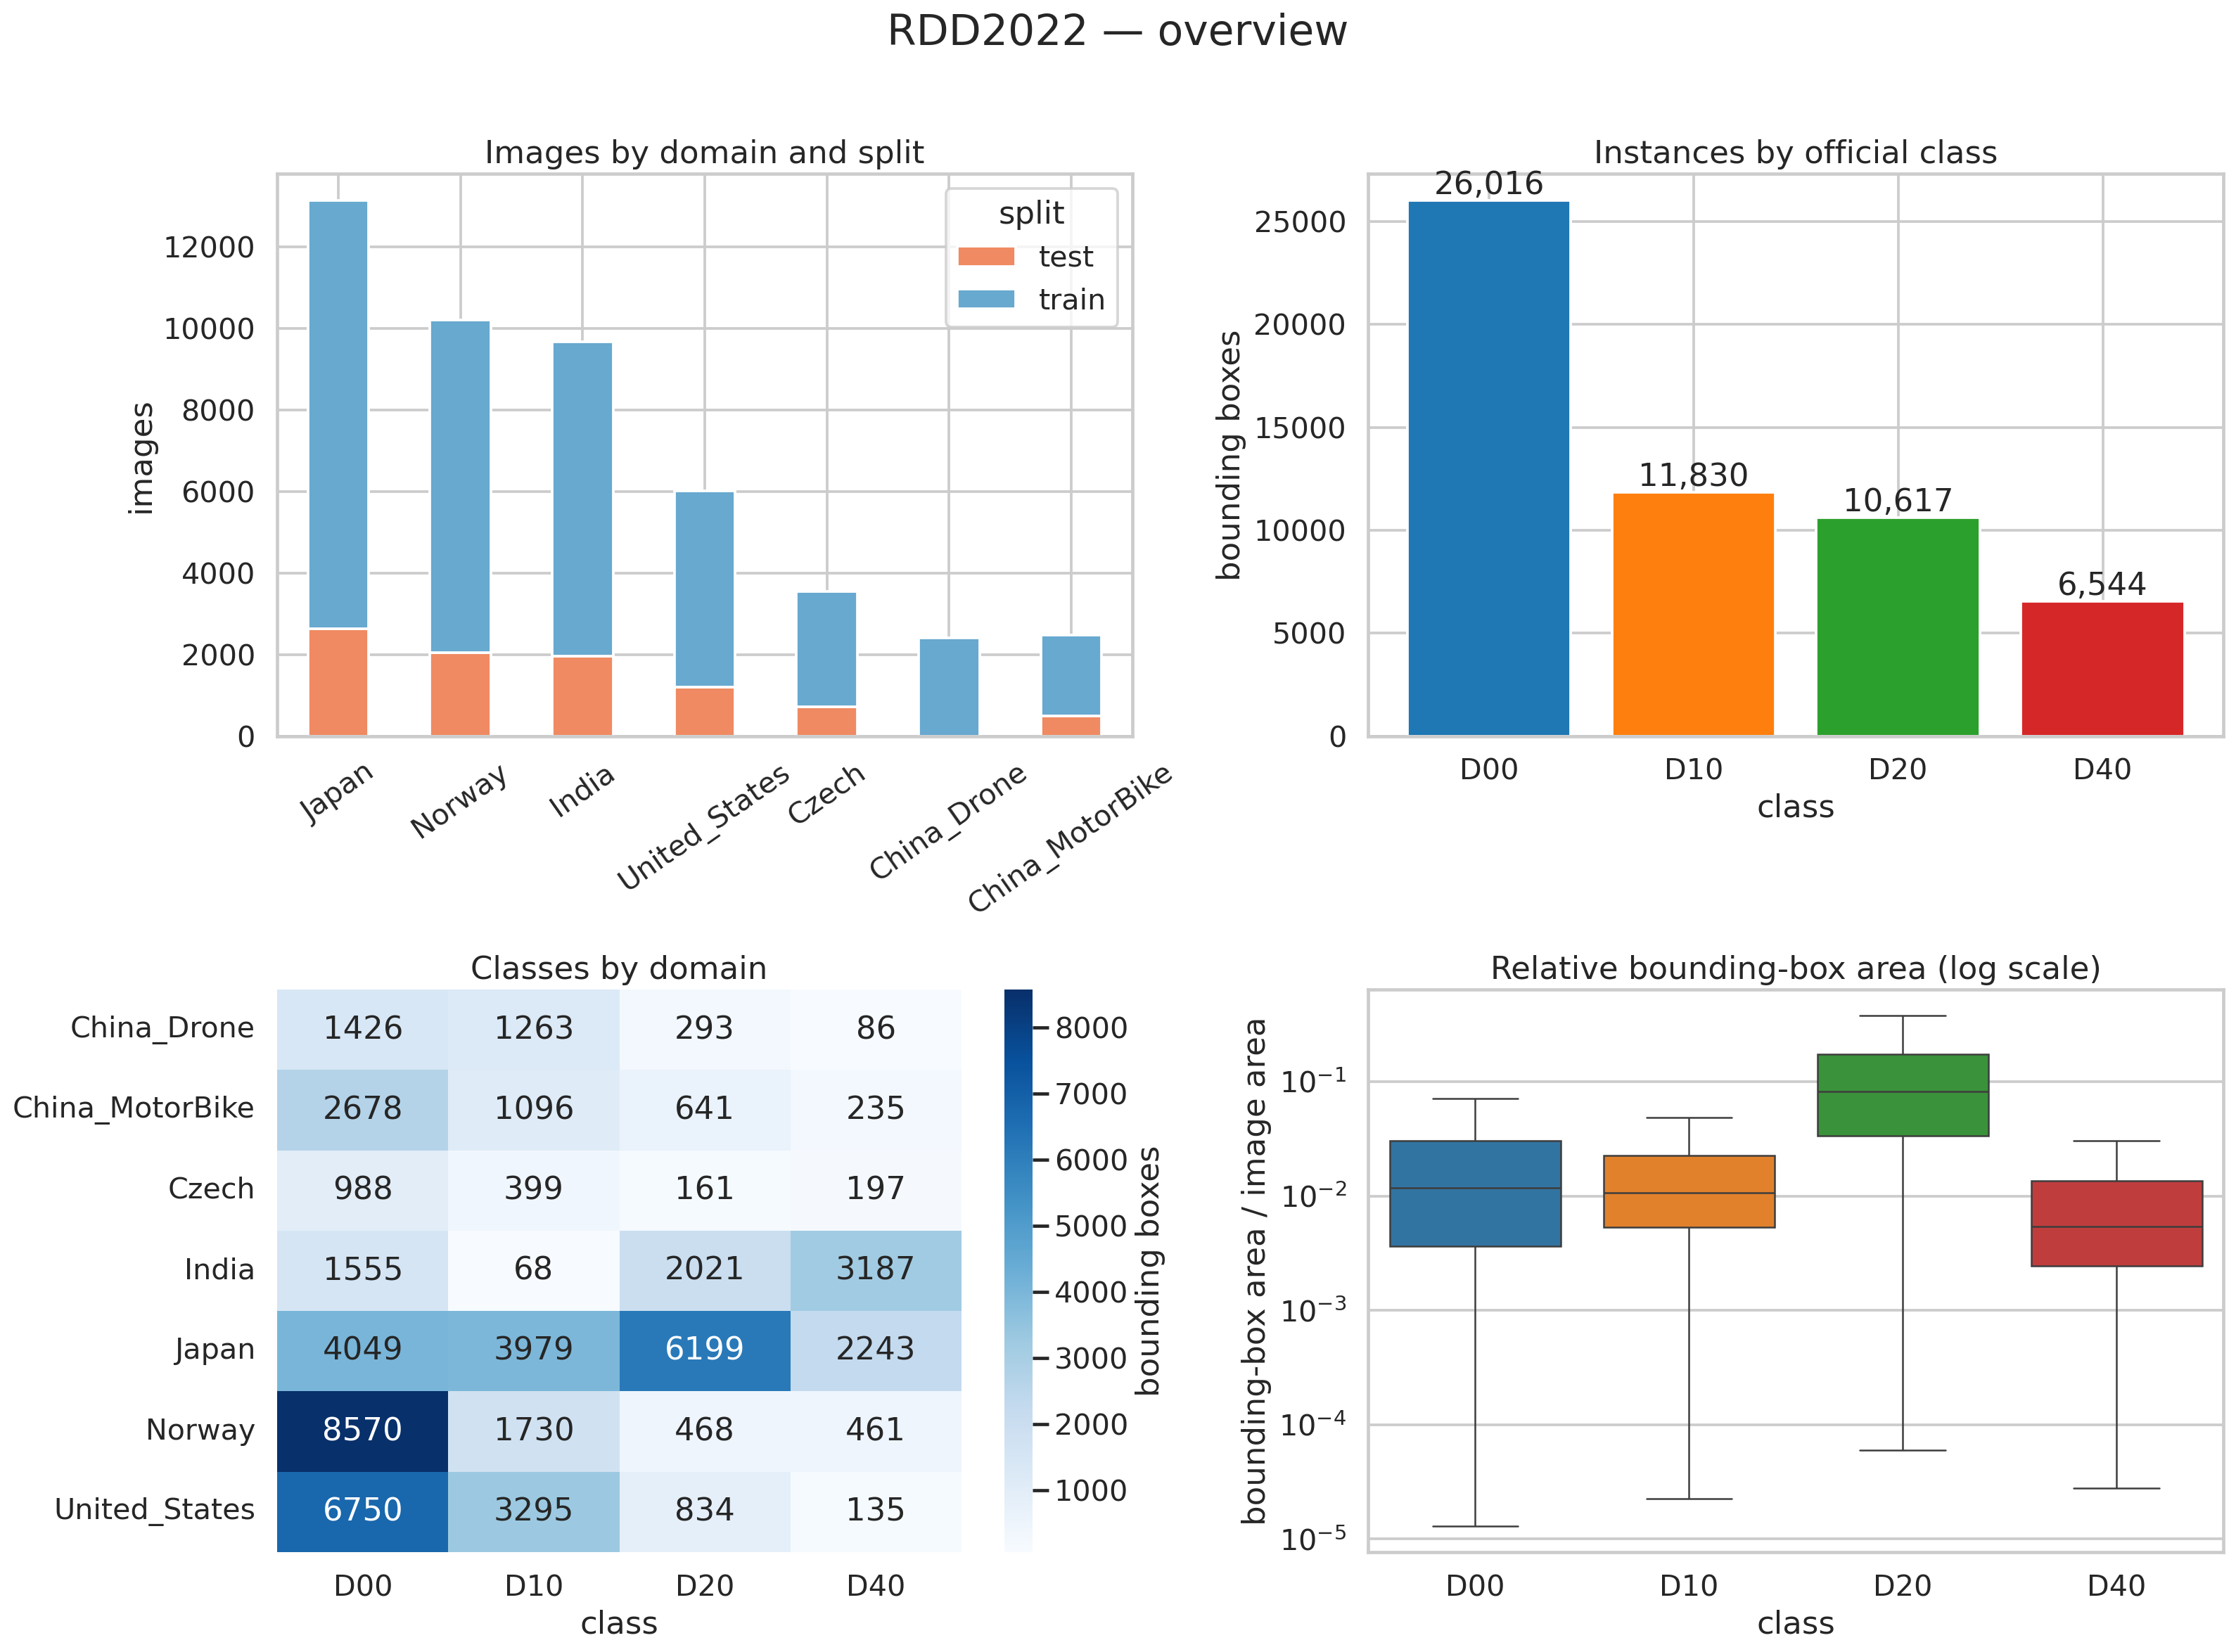
\includegraphics[width=\textwidth]{overview.png}
    \caption{RDD2022 composition, official class frequency, class distribution
    by domain, and relative bounding-box area.}
    \label{fig:eda-overview}
\end{figure*}

\subsection{Class, Scale, and Domain Imbalance}
Table~\ref{tab:class-distribution} summarizes the cleaned official instances.
D00 accounts for nearly half of the annotations, whereas D40 accounts for only
11.9\%. The most frequent class is therefore approximately four times more
common than the least frequent class. Moreover, 41.3\% of valid boxes occupy
less than 1\% of their image area, indicating a substantial small-object
detection challenge.

\begin{table}[t]
    \caption{Official RDD2022 Class Distribution}
    \label{tab:class-distribution}
    \centering
    \begin{tabular}{llrr}
        \toprule
        Class & Damage type & Instances & Share \\
        \midrule
        D00 & Longitudinal crack & 26,016 & 47.3\% \\
        D10 & Transverse crack   & 11,830 & 21.5\% \\
        D20 & Alligator crack    & 10,616 & 19.3\% \\
        D40 & Pothole            &  6,544 & 11.9\% \\
        \bottomrule
    \end{tabular}
\end{table}

Negative-image prevalence also varies sharply by domain. No United States
training image is negative under the four-class definition, compared with
64.3\% of Norway, 62.1\% of the Czech Republic, and 58.2\% of India. This
variation motivates domain-aware reporting and explicit negative sampling.

\section{Data Preparation and Evaluation Protocol}
\label{sec:protocol}

\subsection{Cleaning Rules}
Only D00, D10, D20, and D40 are treated as detection targets. Additional labels
are removed, while images left without an official target are retained as
negative examples. Bounding boxes with non-positive area or coordinates outside
the image are excluded rather than silently clipped. A single canonical
annotation table is used to generate both COCO and YOLO artifacts. The original
unlabeled challenge-test set is kept separate from all internal model selection
and evaluation. Automated validation checks image existence, unique identifiers,
box geometry, normalized YOLO coordinates, COCO references, split membership,
and class mappings. It verified all 38,385 labeled images and 55,006 retained
boxes without a validation failure.

\subsection{Leakage-Aware Internal Split}
Numeric image identifiers are grouped into blocks of 50 consecutive indices.
All images from a block remain in the same subset, reducing leakage from nearby
frames. With seed 2026, blocks are assigned independently within each domain
toward an 80/10/10 train/validation/test target. The deterministic assignment
minimizes a weighted discrepancy in image count, negative images, and instances
of each class, followed by block swaps that improve the same objective without
breaking groups. The resulting split contains 31,021 training, 3,661
validation, and 3,703 internal-test images. No sequence block occurs in more
than one subset.

\begin{table}[t]
    \caption{Clean Internal Split}
    \label{tab:internal-split}
    \centering
    \begin{tabular}{lrrrrr}
        \toprule
        Split & Images & D00 & D10 & D20 & D40 \\
        \midrule
        Train & 31,021 & 20,835 & 9,457 & 8,501 & 5,243 \\
        Validation & 3,661 & 2,588 & 1,190 & 1,054 & 652 \\
        Test & 3,703 & 2,593 & 1,183 & 1,061 & 649 \\
        \bottomrule
    \end{tabular}
\end{table}

\subsection{CPU-Budgeted Training Subset}
The full validation and internal-test partitions are retained, but optimization
uses a deterministic subset of 2,800 training images. Exactly 400 are sampled
from each domain. Within domain $d$, positives and negatives are sampled
separately so the realized negative count equals $\operatorname{round}(400q_d)$.
The resulting subset contains 925 negative images and 4,019 instances: 2,047
D00, 985 D10, 626 D20, and 361 D40. Absolute image lists and realized counts are
stored with seed 2026. Equal quotas implement the risk in
\eqref{eq:balanced-budget} while retaining the substantial domain-specific
difference in background prevalence.

\subsection{Metrics}
The primary metric is COCO average precision averaged over intersection-over-
union thresholds from 0.50 to 0.95 \cite{lin2014coco}. We also report AP50,
AP75, average recall, per-class AP, per-domain AP, and AP for small, medium, and
large objects. Predictions are capped at 100 detections per image for COCO
evaluation. Computational reporting includes latency, throughput, parameter
count, training time, and peak memory measured on fixed hardware. Domain macro
and worst-domain AP use the same shared prediction set. The run is deterministic
at seed 2026, but it is not repeated across seeds; consequently, we report no
unsupported standard deviation and treat training variance as a limitation.

\section{Experimental Setup}
\label{sec:setup}

\subsection{Model Selection}
YOLO11n is the primary compact detector. It has 2.59 million trainable
parameters and is initialized from the official COCO checkpoint. Before the
internal test was accessed, CPU qualification compared it with the official
low-resolution Faster R-CNN MobileNetV3 implementation. Faster R-CNN learned
from negative-only batches but required 2.24~s per two-image optimization batch;
YOLO11n processed eight images in approximately 0.45~s. The former is retained
as an engineering control rather than a commensurate scientific baseline.

\subsection{Training and Model Selection}
The frozen run uses $320\times320$ inputs, batch size 8, and 10 epochs, giving
28,000 image presentations. AdamW uses initial learning rate 0.00125, final
factor 0.05, weight decay $5\times10^{-4}$, and one warm-up epoch. Augmentation
comprises horizontal flipping, HSV perturbation, translation, scaling, and
mosaic, with mosaic disabled for the final two epochs. There is no early
stopping: the final-epoch checkpoint is evaluated on validation, and the
internal test is evaluated once after all choices are frozen.

\subsection{Implementation and Reproducibility}
The run uses Python 3.14.7, PyTorch 2.10.0, TorchVision 0.25.0, and Ultralytics
8.3.203 on an Intel Core i5-10500T CPU with six physical cores, 31~GiB RAM, and
no available CUDA device. Training artifacts record the seed, absolute sample
lists, software versions, model arguments, losses, metrics, and checkpoint
provenance. Integration diagnostics exercised negative-only batches,
serialization, deterministic reruns, and official COCO evaluation; diagnostic
values are excluded from the internal-test table.

\section{Results}
\label{sec:results}

\begin{table}[t]
    \caption{Frozen Internal-Test Result (percent except FPS)}
    \label{tab:main-results}
    \centering
    \begin{tabular}{lrrrr}
        \toprule
        Model & mAP & AP50 & AP75 & FPS \\
        \midrule
        YOLO11n & 3.26 & 8.51 & 1.82 & 43.4 \\
        \bottomrule
    \end{tabular}
\end{table}

Table~\ref{tab:main-results} reports the single frozen evaluation. Training took
1,709.6~s (28.5~min). From the first to the final epoch, classification, box,
and distribution-focal training losses decreased from 3.833 to 2.774, 2.998 to
2.300, and 2.363 to 1.905, respectively. Final validation mAP was 3.01\%, close
to the 3.26\% test result, and no test value was used for model selection.

Scale-stratified AP was 0.26\%, 2.71\%, and 3.63\% for small, medium, and large
objects. AR$_{100}$ reached 27.33\%, showing that the detector often proposed a
nearby candidate but localized or ranked it insufficiently for the stricter AP
integral. By class, mAP/AP50 was 3.83/9.77\% for D00, 3.01/9.17\% for D10,
5.46/12.88\% for D20, and 0.75/2.23\% for D40. Thus, the rare pothole class was
the weakest, whereas alligator cracks were the strongest despite being less
frequent than D00.

Mean preprocessing, inference, and postprocessing time summed to 23.0~ms per
image, or 43.4 images/s for the measured model stages. The complete evaluator,
including file I/O and all pooled, class, and domain COCO computations, took
162.1~s and peaked at 1.33~GiB resident memory. Among 1,414 negative test
images, 13 (0.92\%) produced at least one detection at score 0.25; the mean was
0.0149 detections per negative image. The low false-positive rate therefore
coexists with low recall and AP rather than establishing overall reliability.

\section{Domain-Wise Analysis}
\label{sec:cross-domain}
All domain statistics are computed by slicing one shared internal-test
prediction file. This controls inference settings and prevents domain-specific
threshold tuning. We report pooled, macro, and worst-domain AP according to
\eqref{eq:macro-worst}. Because every domain contributes training images, any
difference reflects within-benchmark heterogeneity, sample composition, and
acquisition difficulty jointly; it does not identify a causal geographic effect
or unseen-domain generalization.

\begin{table}[t]
    \caption{Domain-Sliced Internal-Test Performance}
    \label{tab:domain-results}
    \centering
    \begin{tabular}{lrrr}
        \toprule
        Domain & Images & mAP (\%) & AP50 (\%) \\
        \midrule
        China--drone     & 250   & 5.83 & 16.75 \\
        China--motorbike & 200   & 6.07 & 15.35 \\
        Czech Republic   & 283   & 2.06 &  6.24 \\
        India            & 725   & 0.95 &  2.54 \\
        Japan            & 1,045 & 2.84 &  7.79 \\
        Norway           & 750   & 0.42 &  1.35 \\
        United States    & 450   & 6.11 & 15.11 \\
        \bottomrule
    \end{tabular}
\end{table}

Table~\ref{tab:domain-results} exposes a 14.6-fold range between the United
States and Norway. Domain-macro mAP is 3.47\%, whereas pooled mAP is 3.26\% and
worst-domain mAP is 0.42\%. Equal image quotas did not imply equal positive
supervision: the sampler deliberately preserved each domain's negative-image
rate, which is 64.3\% for Norway but zero for the United States. Acquisition
geometry, resolution, class mix, annotation practice, and test composition are
also confounded with domain, so the table supports a disparity finding but not
a causal geographic explanation.

\section{Ablation Studies}
\label{sec:ablations}
Compute qualification established two useful boundary cases. With a new
four-class head, Faster R-CNN MobileNetV3 produced zero validation AP after 100
steps; at 500 steps it reached 1.25\% mAP and 3.29\% AP50 on a fixed 500-image
validation subset. The equal-domain YOLO11n pilot used 1,400 images for five
epochs and reached 1.75\% mAP and 5.35\% AP50 on all 3,661 validation images in
8.8 minutes of CPU training. These noncommensurate pilots informed model and
budget selection only and are not treated as test-set comparisons. Higher
resolution, tiling, removal of negatives, and repeated seeds remain future
ablations.

\section{Limitations and Discussion}
\label{sec:discussion}
The absolute AP values are not competitive with unconstrained RDD2022 systems.
This is an expected but important boundary result: COCO pretraining cannot
fully compensate for only 28,000 low-resolution image presentations. The
near-monotonic loss reduction and similar validation/test AP suggest budget
underfitting rather than test-specific collapse. Increasing resolution is the
most direct hypothesis for the 0.26\% small-object AP, but it would also raise
CPU cost superlinearly and must be tested rather than assumed.

The current protocol evaluates only the shifts represented in RDD2022 and does
not cover all pavement materials, climates, cameras, or maintenance taxonomies.
Country and sensor are partly confounded---most domains use a characteristic
acquisition setup---so a performance difference cannot be interpreted as a
causal effect of geography alone. Sequence blocks are inferred from numeric
identifiers because timestamps and trajectories are unavailable; grouping
nearby identifiers reduces leakage but cannot guarantee removal of every near
duplicate. Annotation tools and source-specific policies may also contribute
to domain differences. Finally, the official challenge-test labels are not
public, preventing independent evaluation on that split without an external
service. The 320-pixel input is especially restrictive because 41.3\% of boxes
occupy less than 1\% of the original image; resizing can erase fine crack
structure. Equal domain quotas improve representation but depart from natural
deployment prevalence, and only one deterministic training seed is available.
Finally, all evaluated domains occur in training, so the study measures
multidomain performance, not adaptation or generalization to an unseen domain.
Claims are restricted accordingly.

\section{Conclusion}
This study established an auditable CPU-only baseline for multidomain road
damage detection. Sequence-blocked splitting, explicit negative preservation,
and equal-domain sampling prevent common sources of leakage and silent domain
imbalance. YOLO11n completed the frozen 10-epoch run in 28.5 minutes and
processed the test set at 43.4 images/s, but achieved only 3.26\% COCO mAP.
The 14.6-fold domain range, 0.42\% worst-domain mAP, 0.75\% pothole AP, and
0.26\% small-object AP show that computational feasibility does not imply
deployment readiness. The resulting checkpoint is therefore a transparent
lower-compute reference rather than a state-of-the-art claim. Future work
should spend additional compute first on resolution-aware training or tiling,
then test repeated seeds and domain-balanced positive supervision, while
retaining the same untouched sequence-blocked evaluation protocol.

\bibliographystyle{ieee-template/vendor/IEEEtran/bibtex/IEEEtran}
\bibliography{references}

\end{document}
